\icode{E-MI-SI-L2-261031-001}
如图，一小球放置在木板与竖直墙面之间。设墙面对球的压力大小为\(N_1\)，球对木板的压力大小为\(N_2\)。以木板与墙连接	点所形成的水平直线为轴，将木板从图示位置开始缓慢地转到水平位置。不计摩擦，在此过程中\paren[]

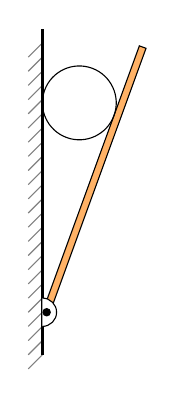
\begin{tikzpicture}[scale=.9,font=\scriptsize]
	\begin{scope}[rotate=70]
		\draw[fill=orange!60] (0,0) rectangle(4,-.1);
		\draw (10:3) circle({3*sin(10)});
	\end{scope}
	\foreach \y in {-.6,-.4,...,4}
		\draw[gray] (0,\y)--++(-.2,-.2);
	\draw[thick] (0,-.6)--(0,4);
	\draw[fill=white] (0,-.2) arc(-90:90:.2);
	\fill (.06,0) circle(.06);
\end{tikzpicture}
\begin{choices}
	\item\(N_1\)始终减小，\(N_2\)始终增大
	\item\(N_1\)始终减小，\(N_2\)始终减小
	\item\(N_1\)先增大后减小，\(N_2\)始终减小
	\item\(N_1\)先增大后减小，\(N_2\)先减小后增大
\end{choices}
\begin{answer}
	B\qquad 提示：

    \begin{tikzpicture}[scale=.9,>=stealth,font=\scriptsize]
	\begin{scope}[rotate=70]
		\draw[fill=orange!60] (0,0) rectangle(4,-.1);
		\draw (10:3)coordinate(o) circle({3*sin(10)});
	\end{scope}
	\foreach \y in {-.6,-.4,...,4}
		\draw[gray] (0,\y)--++(-.2,-.2);
	\draw[thick] (0,-.6)--(0,4);
	\draw[fill=white] (0,-.2) arc(-90:90:.2);
	\fill (.06,0) circle(.06);
    \draw[->] (o)--++(0,-1);
    \draw[->,magenta] (o)--++(160:{1/sin(20)})node[left]{\(N_2\)};
    \draw[->,teal] (o)--++({1/tan(20)},0)node[right]{\(N_1\)};
    \draw[->,teal] ($(o)+(0,-1)$)--++({1/tan(20)},0)coordinate(a);
    \draw[->,magenta] (a)--++(160:{1/sin(20)});
    \draw[->,dashed,magenta] ($(o)+(1,-1)$)--++(135:{sqrt(2)});
    \draw[->,dashed,teal] ($(o)+(0,-1)$)--++(1,0);
\end{tikzpicture}
\end{answer}